\documentclass[12pt]{article}
\usepackage[a4paper,margin=1in]{geometry}
\usepackage{graphicx}
\usepackage{subcaption}
\usepackage{amsmath,amssymb}

\begin{document}

\section*{Two-Site Density-Matrix vs Positive-$P$ Mean Comparison}

\begin{figure}[h]
  \centering
  \begin{subfigure}{0.48\columnwidth}
    \centering
    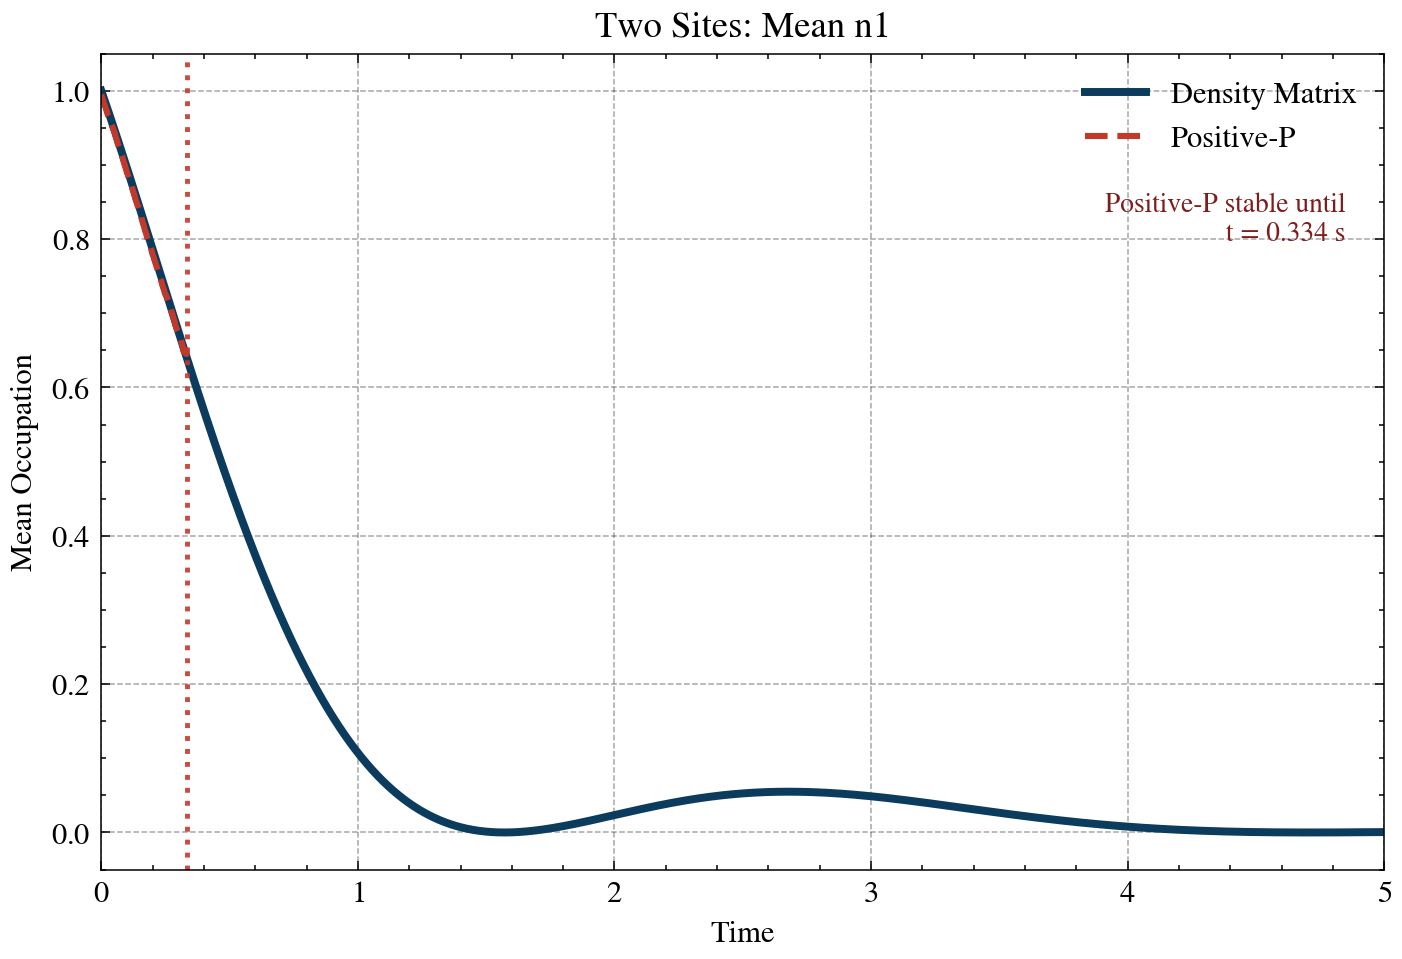
\includegraphics[width=\linewidth]{../../outputs/tmp_density_vs_positivep_mean/figures/two_site_mean_n1_science.png}
    \caption{Site 1 mean occupation for $U=1$.}
    \label{fig:twoSiteU1MeanSite1}
  \end{subfigure}
  \hfill
  \begin{subfigure}{0.48\columnwidth}
    \centering
    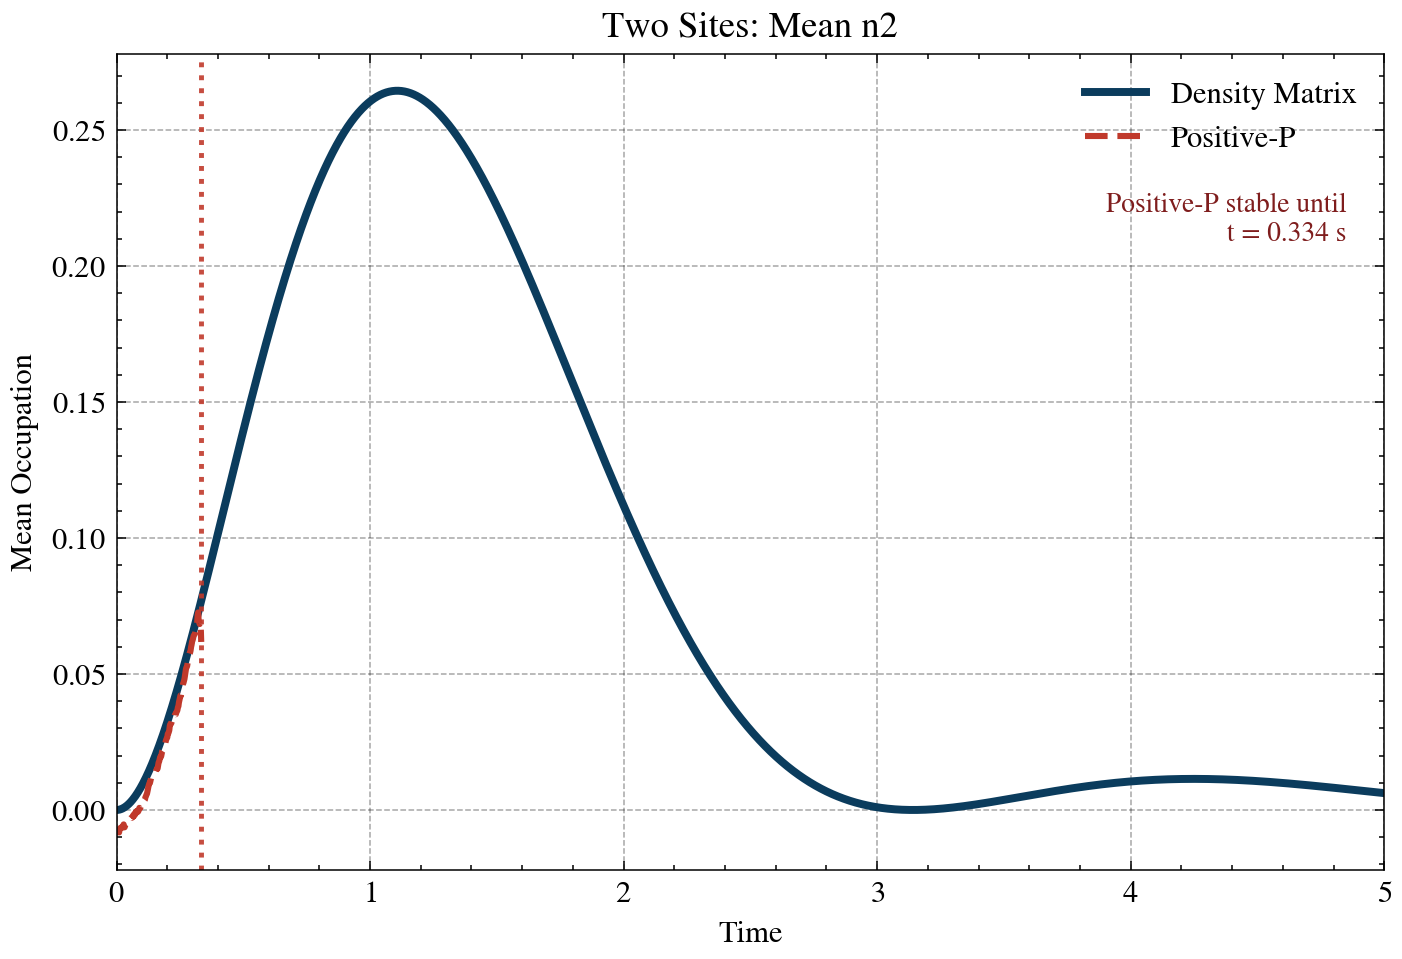
\includegraphics[width=\linewidth]{../../outputs/tmp_density_vs_positivep_mean/figures/two_site_mean_n2_science.png}
    \caption{Site 2 mean occupation for $U=1$.}
    \label{fig:twoSiteU1MeanSite2}
  \end{subfigure}
  \caption{
  Comparison of the density-matrix and positive-$P$ mean occupations for the two-site system with initial Fock state $|1,0\rangle$, interaction strength $U=1$, dissipation rate $\gamma=1$, and hopping amplitude $J=1$. The density-matrix curve is shown over the full $5\,\mathrm{s}$ interval, while the positive-$P$ curve is shown only over its numerically stable time window.
  }
  \label{fig:twoSiteU1MeanComparison}
\end{figure}

\begin{figure}[h]
  \centering
  \begin{subfigure}{0.48\columnwidth}
    \centering
    
\includegraphics[width=\linewidth]{../../outputs/tmp_density_vs_positivep_mean_u0p1/figures/two_site_mean_n1_science.png}
    \caption{Site 1 mean occupation for $U=0.1$.}
    \label{fig:twoSiteU01MeanSite1}
  \end{subfigure}
  \hfill
  \begin{subfigure}{0.48\columnwidth}
    \centering
    
\includegraphics[width=\linewidth]{../../outputs/tmp_density_vs_positivep_mean_u0p1/figures/two_site_mean_n2_science.png}
    \caption{Site 2 mean occupation for $U=0.1$.}
    \label{fig:twoSiteU01MeanSite2}
  \end{subfigure}
  \caption{
  Comparison of the density-matrix and positive-$P$ mean occupations for the two-site system with initial Fock state $|1,0\rangle$, interaction strength $U=0.1$, dissipation rate $\gamma=1$, and hopping amplitude $J=1$. In this weaker-interaction case, the positive-$P$ trajectories remain stable over the full simulated interval.
  }
  \label{fig:twoSiteU01MeanComparison}
\end{figure}

\section*{Discussion Template}

The results in Figs.~\ref{fig:twoSiteU1MeanComparison} and \ref{fig:twoSiteU01MeanComparison} compare the mean site occupations obtained from the density-matrix method and the positive-$P$ method for a two-site Bose-Hubbard system initialized in the Fock state $|1,0\rangle$. In both cases, the density-matrix method provides the reference solution, while the positive-$P$ method is used to test whether the stochastic phase-space approach can reproduce the same mean dynamics.

For the case $U=1$, the positive-$P$ results agree with the density-matrix solution only over an early-time interval. The site-1 occupation decreases from its initially occupied value, while the site-2 occupation rises due to hopping and then decays because of dissipation. However, the annotated cutoff in Fig.~\ref{fig:twoSiteU1MeanComparison} shows that the positive-$P$ simulation remains numerically stable only up to a relatively short time. This indicates that, for the stronger interaction strength, the stochastic trajectories develop large fluctuations quickly enough to limit the useful simulation window.

By contrast, for the weaker interaction $U=0.1$, the positive-$P$ method remains stable over the full $5\,\mathrm{s}$ interval and closely follows the density-matrix reference for both site occupations. This suggests that reducing the interaction strength significantly improves the numerical behavior of the positive-$P$ trajectories for this problem. In this regime, the method is able to reproduce the transport of population from site 1 to site 2 and the subsequent dissipative decay without the premature instability seen in the $U=1$ case.

Taken together, these figures show that the main limitation is not the ability of positive-$P$ to reproduce the short-time mean dynamics, but rather the duration over which the stochastic evolution remains numerically well behaved. The comparison therefore supports the interpretation that positive-$P$ is accurate at short times for both parameter sets, while its practical usefulness depends strongly on the interaction strength.

\end{document}
